%!TEX program = xelatex
\documentclass[UTF8]{ctexart}
\title{你想让你的问题尽快得到解答吗?}
\author{Liam Huang}
\date{\today}

\usepackage{geometry}
\geometry{margin = 1.4in}
\usepackage{xcolor}
\usepackage{amsmath, amssymb}
\usepackage{hologo}
\usepackage{graphicx}
\usepackage{enumitem}
\setlist{noitemsep}
\ifxetex\else
  \usepackage{CJKspace}
\fi
\usepackage{hyperref}
\hypersetup{colorlinks}
\usepackage{etoolbox}
\makeatletter
\patchcmd{\@maketitle}{\LARGE \@title \par}{\Huge \bfseries \@title \par}{}{}
\makeatother

\newcommand{\XeLaTeX}{\hologo{XeLaTeX}}
\newcommand{\pdfLaTeX}{\hologo{pdfLaTeX}}
\renewcommand{\CTeX}{\ensuremath{\mathbb{C}}\!\TeX}
\newcommand{\mdesc}[1]{{\sffamily\kaishu\color{red} #1}}
\newcommand{\myem}[1]{{\bfseries\color{red} #1}}
\newcommand{\myemph}[1]{{\sffamily\kaishu\color{red!80!orange} #1}}
\newcommand{\Warning}{\myem{\Large \rule{0pt}{1.4em}不耐心看完文档的话就没人回答你的问题哦}}
\newcommand{\warning}{\cleaders\hbox to \linewidth{\hss\Warning\hss}\vfill}

\begin{document}
\maketitle
\warning
\clearpage
\section{提问模板} % (fold)
\label{sec:question_template}
这里给出两个基本的提问模板,相关内容如何填写请参照后文。
\subsection{编译遇到错误} % (fold)
\label{sub:qt_error}
如果你在编译的时候遇到错误,请参照下面的模板提问。

\begin{center}
\fbox{\begin{minipage}{.9\linewidth}
  我编译遇到了错误,请问应该如何解决?是否还需要提供更多信息?谢谢!\par
  编译报错:\par
  \mdesc{这里填入编译报错信息的{\bfseries 截图}\par(报错信息通常是从一个行首的叹号开始,到一个行首的问号结束)}\par
  我的代码是:\par
  \mdesc{这里填入 MWE,{\bfseries 请勿截图}}\par
  我使用的 \TeX{} 发行版是:\par
  \mdesc{\TeX Live|Mac\TeX{}|MiK\TeX{}|\CTeX}\par
  我的文档编码是:\par
  \mdesc{UTF-8|GBK}\par
  我使用的编译方式是:\par
  \mdesc{\XeLaTeX{}|\pdfLaTeX{}|\LaTeX{}}
\end{minipage}}
\end{center}
% subsection qt_error (end)
\subsection{编译结果不符合期望} % (fold)
\label{sub:qt_expection}
如果你编译的过程中没有遇到错误,但是编译出的 PDF 文档效果不满意,请参照下面的模板提问。

\begin{center}
\fbox{\begin{minipage}{.9\linewidth}
  我编译之后效果不对,请问应该如何解决?是否还需要提供更多信息?谢谢!\par
  当前效果:\par
  \mdesc{相应 PDF 截图}\par
  预期效果:\par
  \mdesc{对效果的精准描述,或是预期效果截图}\par
  我的代码是:\par
  \mdesc{这里填入 MWE,{\bfseries 请勿截图}}\par
  我使用的 \TeX{} 发行版是:\par
  \mdesc{\TeX Live|Mac\TeX{}|MiK\TeX{}|\CTeX}\par
  我的文档编码是:\par
  \mdesc{UTF-8|GBK}\par
  我使用的编译方式是:\par
  \mdesc{\XeLaTeX{}|\pdfLaTeX{}|\LaTeX{}}
\end{minipage}}
\end{center}
% subsection qt_expection (end)
% section question_template (end)
\section{提问之前,你应该做的事情} % (fold)
\label{sec:before_question}
\paragraph{查阅文档} % (fold)
\label{par:RTFM}
大多数的问题,文档都能为你提供标准的解答。因此在你提问之前,你最好先去阅读一下相关的文档,至少确保你阅读过一份完整的入门文档\footnote{\url{http://zip.liam0205.me}}。如果你能够在你提问的同时表明自己已经阅读过文档, 但是依旧留有困惑,潜在的回答者会更加愿意为你解答。如果你不知道如何寻找文档,请阅读下面的「新手请先读我」。

中文 \TeX{} 社区两个著名的文档:\href{http://bbs.ctex.org/forum.php?mod=viewthread&tid=48244}{新手请先读我}、\href{https://liam0205.me/uploads/LaTeX/ChinaTeXMathFAQ_V1.1.pdf}{China\TeX{} Math FAQ}。
% paragraph RTFM (end)
\paragraph{检索互联网} % (fold)
\label{par:STFW}
\TeX{} 是一个成熟而经典的工具,人们使用它已有三十多年。初学者遇到的绝大部分问题都能够在互联网上找到成熟的答案。你最好是先在互联网上检索,再进行提问。

需要注意的是,虽然 \TeX{} 和 \LaTeX{} 是成熟稳定的工具,但是一些相关技术,特别是中文支持技术却在不断发生变化。如果你在网络上检索的资料涉及到这部分过时的内容,请务必小心行事。比如涉及到 \textsf{CJK} 以及相关宏包的用法的资料,基本可以认定为过时。

中文 \TeX{} 社区:\href{http://bbs.ctex.org}{\CTeX{} 论坛}、\href{http://bbs.chinatex.org}{China\TeX{} 论坛}、\href{http://www.newsmth.net/nForum/#!board/TeX}{水木社区 \TeX/\LaTeX{} 板块}、\href{http://www.latexstudio.net}{\LaTeX{}studio 网站}。

此外,\href{https://liam0205.me}{Liam Huang 的博客}上也有许多\href{https://liam0205.me/categories/LaTeX/}{关于 \LaTeX{} 的文章}。
% paragraph STFW (end)
% section before_question (end)
\section{提问之时,给你的一些建议} % (fold)
\label{sec:during_questioning}
\paragraph{整理 MWE} % (fold)
\label{par:_mwe}
MWE 是 Minimal Working Example 的缩写,意思是「最小工作示例」。顾名思义,最小工作示例的特点有三:
\begin{description}
  \item[简短] 不包含与问题无关的代码片段;
  \item[工作] 能够独立运行于他人的计算机上,而不需要再添加额外的代码;
  \item[示例] 在他人计算机上的运行结果,能完整地再现你所遇到的问题。
\end{description}

希望他人帮忙解决问题,首先要做的就是让他们理解你遇到了什么问题。因此\myemph{示例}必不可少。

如果提供的示例在他人的计算机上无法运行,那么他们也就没有办法知道你遇到了什么问题。所以提供的代码必须能够正常\myemph{工作}。

时间对任何人都是一笔宝贵的财富。如果提供的代码冗长,则回答者势必要花费大量时间阅读不必要的代码。这浪费了回答者的时间,也浪费了提问者的时间(需要等待更久)。因此有必要让示例足够\myemph{简短}。

\paragraph{给出完整准确的错误提示} % (fold)
\label{par:Err_message}
\LaTeX{} 的错误提示分成四个部分,我们用一个例子来解释这四个部分分别是什么。

\medskip

\hskip -1.2in\hbox to 0pt{\begin{minipage}[b]{.33\linewidth}
\begin{verbatim}
\documentclass{minimal}
\begin{document}
\usepackage{amsmath}
\end{document}
\end{verbatim}\end{minipage}}\hfill\raisebox{-.5ex}{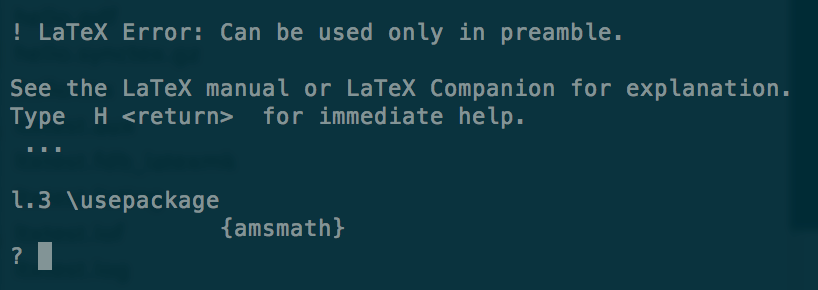
\includegraphics[scale = 0.8]{err_msg.png}}

右边截图是左边代码编译时的报错。其中:
\begin{description}[align = right,
  leftmargin = 2\ccwd, itemindent = 0pt, labelwidth = 5\ccwd]
  \item[错误名称] 以叹号开头的行说明出错原因,示例中提示:「\LaTeX{} 错误:只能用在导言区」。
  \item[提示建议] 中间段落是 \LaTeX{} 给出的提示建议。
  \item[出错位置] 以字母 \texttt{l} 开头的那一行给出出错的具体位置。可以看到代码在 \verb|\usepackage| 之后截断分为两行,这说明问题出在截断。这里是第三行的 \verb|\usepackage| 出错了。
  \item[询问提示符] 以问号开头的行,表示 \LaTeX{} 正在等待用户输入。
\end{description}

综合可得:「第三行的 \verb|\usepackage| 只能放在导言区,不能放在正文部分」。

\myemph{\bfseries 错误截图应该总是全部四个部分,即从叹号开始,到问号结束。}
% paragraph Err_message (end)
% \clearpage
\paragraph{提问者常犯的错误} % (fold)
\label{subp:Frequant_Problems}
提问者常犯的错误有三:一是只提供代码截图;二是只提供代码片段;三是代码冗余不加删节。

\subparagraph{\myemph{永远不要提供代码截图,请直接提供代码原文}}\LaTeX{} 是非常精确的系统。这份精确同时也意味着复杂。除了一些经典的问题,大多数问题通常无法「看一眼」就解决。这意味着,回答者通常需要在他们自己的计算机上运行你的代码。如果你只是给出了代码截图,回答者就不得不自己在计算机上重复输入你的代码。浪费时间不说,通常也不会有人乐意这么做。

\subparagraph{\myemph{永远不要只提供代码片段,请提供完整的工作示例}}我们知道,如果一个人感冒流涕,他不会只把自己的鼻子送给医生去检查。\LaTeX{} 代码也一样。如果一段代码出现问题,你也不能只提供这一部分的代码片段,问题有可能出在别的地方。如果你只提供代码片段,大多数的问题是无从解决的。

\subparagraph{\myemph{永远不要提供不加删节的冗长代码,请提供简短的工作示例}}也有的人,会将未做删节的代码一股脑全部丢给别人。要知道,所有的人都是在工作学习之余帮你解决问题的;而没有人乐意在休息时间阅读\emph{一段乱码}。
% subparagraph Frequant_Problems (end)
% paragraph _mwe (end)
% section during_questioning (end)
\section{提问的智慧} % (fold)
\label{sec:Smart_question}
这是一篇最先由 Eric Steven Raymond 撰写的文档,说明了提问者应当如何提问,使得回答者能 够更容易理解并能使提问者学到更多东西。

参见它的\href{http://www.catb.org/~esr/faqs/smart-questions.html}{英文原版}和\href{https://github.com/ryanhanwu/How-To-Ask-Questions-The-Smart-Way}{中文译文}。
% section Smart_question (end)
\end{document}
